\chapter{Chapter XXII}

\begin{verse}
My daughter--O my ducats--O my daughter!\\
------O my Christian ducats!\\
Justice--the Law--my ducats, and my daughter!\\!
\attrib{--Merchant of Venice}
\end{verse}

\lettrine{L}{eaving} the Saxon chiefs to return to their banquet as
soon as their
ungratified curiosity should permit them to attend to the calls of their
half-satiated appetite, we have to look in upon the yet more severe
imprisonment of Isaac of York. The poor Jew had been hastily thrust into
a dungeon-vault of the castle, the floor of which was deep beneath the
level of the ground, and very damp, being lower than even the moat
itself. The only light was received through one or two loop-holes far
above the reach of the captive's hand. These apertures admitted, even at
mid-day, only a dim and uncertain light, which was changed for utter
darkness long before the rest of the castle had lost the blessing of
day. Chains and shackles, which had been the portion of former captives,
from whom active exertions to escape had been apprehended, hung rusted
and empty on the walls of the prison, and in the rings of one of those
sets of fetters there remained two mouldering bones, which seemed to
have been once those of the human leg, as if some prisoner had been left
not only to perish there, but to be consumed to a skeleton.

At one end of this ghastly apartment was a large fire-grate, over the
top of which were stretched some transverse iron bars, half devoured
with rust.

The whole appearance of the dungeon might have appalled a stouter heart
than that of Isaac, who, nevertheless, was more composed under the
imminent pressure of danger, than he had seemed to be while affected by
terrors, of which the cause was as yet remote and contingent. The lovers
of the chase say that the hare feels more agony during the pursuit of
the greyhounds, than when she is struggling in their fangs.\footnote{``Nota
Bene.''--We by no means warrant the accuracy of
this piece of natural history, which we give on the authority of the
Wardour MS. L. T.}

And thus it is probable, that the Jews, by the very frequency of their
fear on all occasions, had their minds in some degree prepared for every
effort of tyranny which could be practised upon them; so that no
aggression, when it had taken place, could bring with it that surprise
which is the most disabling quality of terror. Neither was it the first
time that Isaac had been placed in circumstances so dangerous. He had
therefore experience to guide him, as well as hope, that he might again,
as formerly, be delivered as a prey from the fowler. Above all, he had
upon his side the unyielding obstinacy of his nation, and that unbending
resolution, with which Israelites have been frequently known to submit
to the uttermost evils which power and violence can inflict upon them,
rather than gratify their oppressors by granting their demands.

In this humour of passive resistance, and with his garment collected
beneath him to keep his limbs from the wet pavement, Isaac sat in a
corner of his dungeon, where his folded hands, his dishevelled hair and
beard, his furred cloak and high cap, seen by the wiry and broken light,
would have afforded a study for Rembrandt, had that celebrated painter
existed at the period. The Jew remained, without altering his position,
for nearly three hours, at the expiry of which steps were heard on the
dungeon stair. The bolts screamed as they were withdrawn--the hinges
creaked as the wicket opened, and Reginald Front-de-Boeuf, followed by
the two Saracen slaves of the Templar, entered the prison.

Front-de-Boeuf, a tall and strong man, whose life had been spent in
public war or in private feuds and broils, and who had hesitated at no
means of extending his feudal power, had features corresponding to his
character, and which strongly expressed the fiercer and more malignant
passions of the mind. The scars with which his visage was seamed, would,
on features of a different cast, have excited the sympathy and
veneration due to the marks of honourable valour; but, in the peculiar
case of Front-de-Boeuf, they only added to the ferocity of his
countenance, and to the dread which his presence inspired. This
formidable baron was clad in a leathern doublet, fitted close to his
body, which was frayed and soiled with the stains of his armour. He had
no weapon, excepting a poniard at his belt, which served to
counterbalance the weight of the bunch of rusty keys that hung at his
right side.

The black slaves who attended Front-de-Boeuf were stripped of their
gorgeous apparel, and attired in jerkins and trowsers of coarse linen,
their sleeves being tucked up above the elbow, like those of butchers
when about to exercise their function in the slaughter-house. Each had
in his hand a small pannier; and, when they entered the dungeon, they
stopt at the door until Front-de-Boeuf himself carefully locked and
double-locked it. Having taken this precaution, he advanced slowly up
the apartment towards the Jew, upon whom he kept his eye fixed, as if he
wished to paralyze him with his glance, as some animals are said to
fascinate their prey. It seemed indeed as if the sullen and malignant
eye of Front-de-Boeuf possessed some portion of that supposed power over
his unfortunate prisoner. The Jew sat with his mouth agape, and his eyes
fixed on the savage baron with such earnestness of terror, that his
frame seemed literally to shrink together, and to diminish in size while
encountering the fierce Norman's fixed and baleful gaze. The unhappy
Isaac was deprived not only of the power of rising to make the obeisance
which his terror dictated, but he could not even doff his cap, or utter
any word of supplication; so strongly was he agitated by the conviction
that tortures and death were impending over him.

On the other hand, the stately form of the Norman appeared to dilate in
magnitude, like that of the eagle, which ruffles up its plumage when
about to pounce on its defenceless prey. He paused within three steps of
the corner in which the unfortunate Jew had now, as it were, coiled
himself up into the smallest possible space, and made a sign for one of
the slaves to approach. The black satellite came forward accordingly,
and, producing from his basket a large pair of scales and several
weights, he laid them at the feet of Front-de-Boeuf, and again retired
to the respectful distance, at which his companion had already taken his
station.

The motions of these men were slow and solemn, as if there impended over
their souls some preconception of horror and of cruelty. Front-de-Boeuf
himself opened the scene by thus addressing his ill-fated captive.

``Most accursed dog of an accursed race,'' he said, awaking with his
deep and sullen voice the sullen echoes of his dungeon vault, ``seest
thou these scales?''

The unhappy Jew returned a feeble affirmative.

``In these very scales shalt thou weigh me out,'' said the relentless
Baron, ``a thousand silver pounds, after the just measure and weight of
the Tower of London.''

``Holy Abraham!'' returned the Jew, finding voice through the very
extremity of his danger, ``heard man ever such a demand?--Who ever
heard, even in a minstrel's tale, of such a sum as a thousand pounds of
silver?--What human sight was ever blessed with the vision of such a
mass of treasure?--Not within the walls of York, ransack my house and
that of all my tribe, wilt thou find the tithe of that huge sum of
silver that thou speakest of.''

``I am reasonable,'' answered Front-de-Boeuf, ``and if silver be scant,
I refuse not gold. At the rate of a mark of gold for each six pounds of
silver, thou shalt free thy unbelieving carcass from such punishment as
thy heart has never even conceived.''

``Have mercy on me, noble knight!'' exclaimed Isaac; ``I am old, and
poor, and helpless. It were unworthy to triumph over me--It is a poor
deed to crush a worm.''

``Old thou mayst be,'' replied the knight; ``more shame to their folly
who have suffered thee to grow grey in usury and knavery--Feeble thou
mayst be, for when had a Jew either heart or hand--But rich it is well
known thou art.''

``I swear to you, noble knight,'' said the Jew ``by all which I believe,
and by all which we believe in common---''

``Perjure not thyself,'' said the Norman, interrupting him, ``and let
not thine obstinacy seal thy doom, until thou hast seen and well
considered the fate that awaits thee. Think not I speak to thee only to
excite thy terror, and practise on the base cowardice thou hast derived
from thy tribe. I swear to thee by that which thou dost NOT believe, by
the gospel which our church teaches, and by the keys which are given her
to bind and to loose, that my purpose is deep and peremptory. This
dungeon is no place for trifling. Prisoners ten thousand times more
distinguished than thou have died within these walls, and their fate
hath never been known! But for thee is reserved a long and lingering
death, to which theirs were luxury.''

He again made a signal for the slaves to approach, and spoke to them
apart, in their own language; for he also had been in Palestine, where
perhaps, he had learnt his lesson of cruelty. The Saracens produced from
their baskets a quantity of charcoal, a pair of bellows, and a flask of
oil. While the one struck a light with a flint and steel, the other
disposed the charcoal in the large rusty grate which we have already
mentioned, and exercised the bellows until the fuel came to a red glow.

``Seest thou, Isaac,'' said Front-de-Boeuf, ``the range of iron bars
above the glowing charcoal?\footnote{Note E. The range of iron bars
above that glowing
charcoal. See page~\pageref{noteCXXII}.}--on that warm couch thou shalt
lie, stripped of thy clothes as if thou wert to rest on a bed of down.
One of these slaves shall maintain the fire beneath thee, while the
other shall anoint thy wretched limbs with oil, lest the roast should
burn.--Now, choose betwixt such a scorching bed and the payment of a
thousand pounds of silver; for, by the head of my father, thou hast no
other option.''

\begin{figure}
    \centering
    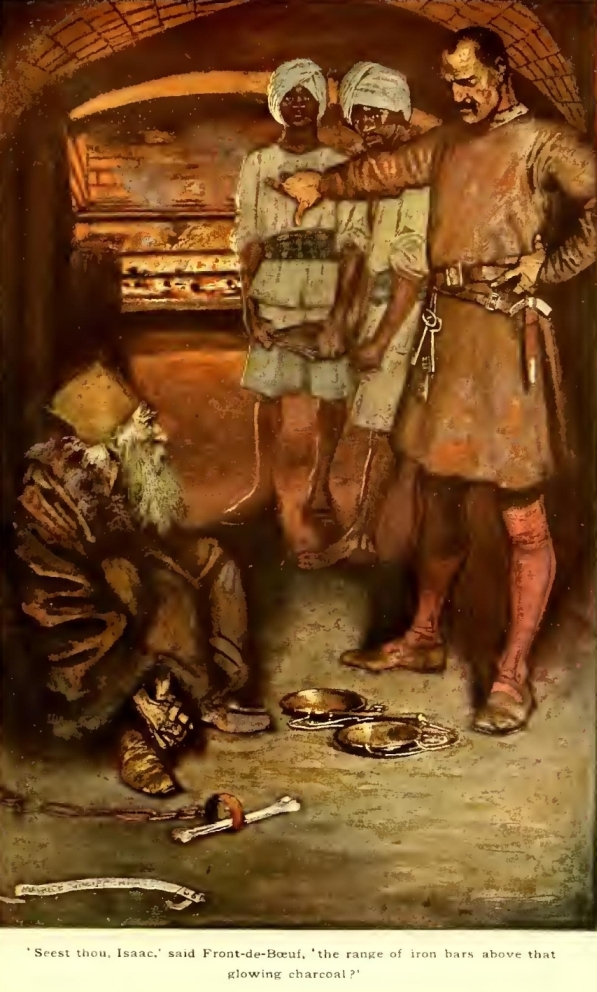
\includegraphics[height=.9\textheight]{ivanhoe/0285m}
    \caption{`Seest though, Isaac,' said Front-de-Boeuf, `the range of
    iron bars above that glowing charcoal?'}
\end{figure}

``It is impossible,'' exclaimed the miserable Jew--``it is impossible
that your purpose can be real! The good God of nature never made a heart
capable of exercising such cruelty!''

``Trust not to that, Isaac,'' said Front-de-Boeuf, ``it were a fatal
error. Dost thou think that I, who have seen a town sacked, in which
thousands of my Christian countrymen perished by sword, by flood, and by
fire, will blench from my purpose for the outcries or screams of one
single wretched Jew?--or thinkest thou that these swarthy slaves, who
have neither law, country, nor conscience, but their master's will--who
use the poison, or the stake, or the poniard, or the cord, at his
slightest wink--thinkest thou that THEY will have mercy, who do not even
understand the language in which it is asked?--Be wise, old man;
discharge thyself of a portion of thy superfluous wealth; repay to the
hands of a Christian a part of what thou hast acquired by the usury thou
hast practised on those of his religion. Thy cunning may soon swell out
once more thy shrivelled purse, but neither leech nor medicine can
restore thy scorched hide and flesh wert thou once stretched on these
bars. Tell down thy ransom, I say, and rejoice that at such rate thou
canst redeem thee from a dungeon, the secrets of which few have returned
to tell. I waste no more words with thee--choose between thy dross and
thy flesh and blood, and as thou choosest, so shall it be.''

``So may Abraham, Jacob, and all the fathers of our people assist me,''
said Isaac, ``I cannot make the choice, because I have not the means of
satisfying your exorbitant demand!''

``Seize him and strip him, slaves,'' said the knight, ``and let the
fathers of his race assist him if they can.''

The assistants, taking their directions more from the Baron's eye and
his hand than his tongue, once more stepped forward, laid hands on the
unfortunate Isaac, plucked him up from the ground, and, holding him
between them, waited the hard-hearted Baron's farther signal. The
unhappy Jew eyed their countenances and that of Front-de-Boeuf, in hope
of discovering some symptoms of relenting; but that of the Baron
exhibited the same cold, half-sullen, half-sarcastic smile which had
been the prelude to his cruelty; and the savage eyes of the Saracens,
rolling gloomily under their dark brows, acquiring a yet more sinister
expression by the whiteness of the circle which surrounds the pupil,
evinced rather the secret pleasure which they expected from the
approaching scene, than any reluctance to be its directors or agents.
The Jew then looked at the glowing furnace, over which he was presently
to be stretched, and seeing no chance of his tormentor's relenting, his
resolution gave way.

``I will pay,'' he said, ``the thousand pounds of silver--That is,'' he
added, after a moment's pause, ``I will pay it with the help of my
brethren; for I must beg as a mendicant at the door of our synagogue ere
I make up so unheard-of a sum.--When and where must it be delivered?''

``Here,'' replied Front-de-Boeuf, ``here it must be delivered--weighed
it must be--weighed and told down on this very dungeon floor.--Thinkest
thou I will part with thee until thy ransom is secure?''

``And what is to be my surety,'' said the Jew, ``that I shall be at
liberty after this ransom is paid?''

``The word of a Norman noble, thou pawn-broking slave,'' answered
Front-de-Boeuf; ``the faith of a Norman nobleman, more pure than the
gold and silver of thee and all thy tribe.''

``I crave pardon, noble lord,'' said Isaac timidly, ``but wherefore
should I rely wholly on the word of one who will trust nothing to
mine?''

``Because thou canst not help it, Jew,'' said the knight, sternly.
``Wert thou now in thy treasure-chamber at York, and were I craving a
loan of thy shekels, it would be thine to dictate the time of payment,
and the pledge of security. This is MY treasure-chamber. Here I have
thee at advantage, nor will I again deign to repeat the terms on which I
grant thee liberty.''

The Jew groaned deeply.--``Grant me,'' he said, ``at least with my own
liberty, that of the companions with whom I travel. They scorned me as a
Jew, yet they pitied my desolation, and because they tarried to aid me
by the way, a share of my evil hath come upon them; moreover, they may
contribute in some sort to my ransom.''

``If thou meanest yonder Saxon churls,'' said Front-de-Boeuf, ``their
ransom will depend upon other terms than thine. Mind thine own concerns,
Jew, I warn thee, and meddle not with those of others.''

``I am, then,'' said Isaac, ``only to be set at liberty, together with
mine wounded friend?''

``Shall I twice recommend it,'' said Front-de-Boeuf, ``to a son of
Israel, to meddle with his own concerns, and leave those of others
alone?--Since thou hast made thy choice, it remains but that thou payest
down thy ransom, and that at a short day.''

``Yet hear me,'' said the Jew--``for the sake of that very wealth which
thou wouldst obtain at the expense of thy---'' Here he stopt short,
afraid of irritating the savage Norman. But Front-de-Boeuf only laughed,
and himself filled up the blank at which the Jew had hesitated.

``At the expense of my conscience, thou wouldst say, Isaac; speak it
out--I tell thee, I am reasonable. I can bear the reproaches of a loser,
even when that loser is a Jew. Thou wert not so patient, Isaac, when
thou didst invoke justice against Jacques Fitzdotterel, for calling thee
a usurious blood-sucker, when thy exactions had devoured his
patrimony.''

``I swear by the Talmud,'' said the Jew, ``that your valour has been
misled in that matter. Fitzdotterel drew his poniard upon me in mine own
chamber, because I craved him for mine own silver. The term of payment
was due at the Passover.''

``I care not what he did,'' said Front-de-Boeuf; ``the question is, when
shall I have mine own?--when shall I have the shekels, Isaac?''

``Let my daughter Rebecca go forth to York,'' answered Isaac, ``with
your safe conduct, noble knight, and so soon as man and horse can
return, the treasure---'' Here he groaned deeply, but added, after the
pause of a few seconds,--``The treasure shall be told down on this very
floor.''

``Thy daughter!'' said Front-de-Boeuf, as if surprised,--``By heavens,
Isaac, I would I had known of this. I deemed that yonder black-browed
girl had been thy concubine, and I gave her to be a handmaiden to Sir
Brian de Bois-Guilbert, after the fashion of patriarchs and heroes of
the days of old, who set us in these matters a wholesome example.''

The yell which Isaac raised at this unfeeling communication made the
very vault to ring, and astounded the two Saracens so much that they let
go their hold of the Jew. He availed himself of his enlargement to throw
himself on the pavement, and clasp the knees of Front-de-Boeuf.

``Take all that you have asked,'' said he, ``Sir Knight--take ten times
more--reduce me to ruin and to beggary, if thou wilt,--nay, pierce me
with thy poniard, broil me on that furnace, but spare my daughter,
deliver her in safety and honour!--As thou art born of woman, spare the
honour of a helpless maiden--She is the image of my deceased Rachel, she
is the last of six pledges of her love--Will you deprive a widowed
husband of his sole remaining comfort?--Will you reduce a father to wish
that his only living child were laid beside her dead mother, in the tomb
of our fathers?''

``I would,'' said the Norman, somewhat relenting, ``that I had known of
this before. I thought your race had loved nothing save their
moneybags.''

``Think not so vilely of us, Jews though we be,'' said Isaac, eager to
improve the moment of apparent sympathy; ``the hunted fox, the tortured
wildcat loves its young--the despised and persecuted race of Abraham
love their children!''

``Be it so,'' said Front-de-Boeuf; ``I will believe it in future, Isaac,
for thy very sake--but it aids us not now, I cannot help what has
happened, or what is to follow; my word is passed to my comrade in arms,
nor would I break it for ten Jews and Jewesses to boot. Besides, why
shouldst thou think evil is to come to the girl, even if she became
Bois-Guilbert's booty?''

``There will, there must!'' exclaimed Isaac, wringing his hands in
agony; ``when did Templars breathe aught but cruelty to men, and
dishonour to women!''

``Dog of an infidel,'' said Front-de-Boeuf, with sparkling eyes, and not
sorry, perhaps, to seize a pretext for working himself into a passion,
``blaspheme not the Holy Order of the Temple of Zion, but take thought
instead to pay me the ransom thou hast promised, or woe betide thy
Jewish throat!''

``Robber and villain!'' said the Jew, retorting the insults of his
oppressor with passion, which, however impotent, he now found it
impossible to bridle, ``I will pay thee nothing--not one silver penny
will I pay thee, unless my daughter is delivered to me in safety and
honour!''

``Art thou in thy senses, Israelite?'' said the Norman, sternly--``has
thy flesh and blood a charm against heated iron and scalding oil?''

``I care not!'' said the Jew, rendered desperate by paternal affection;
``do thy worst. My daughter is my flesh and blood, dearer to me a
thousand times than those limbs which thy cruelty threatens. No silver
will I give thee, unless I were to pour it molten down thy avaricious
throat--no, not a silver penny will I give thee, Nazarene, were it to
save thee from the deep damnation thy whole life has merited! Take my
life if thou wilt, and say, the Jew, amidst his tortures, knew how to
disappoint the Christian.''

``We shall see that,'' said Front-de-Boeuf; ``for by the blessed rood,
which is the abomination of thy accursed tribe, thou shalt feel the
extremities of fire and steel!--Strip him, slaves, and chain him down
upon the bars.''

In spite of the feeble struggles of the old man, the Saracens had
already torn from him his upper garment, and were proceeding totally to
disrobe him, when the sound of a bugle, twice winded without the castle,
penetrated even to the recesses of the dungeon, and immediately after
loud voices were heard calling for Sir Reginald Front-de-Boeuf.
Unwilling to be found engaged in his hellish occupation, the savage
Baron gave the slaves a signal to restore Isaac's garment, and, quitting
the dungeon with his attendants, he left the Jew to thank God for his
own deliverance, or to lament over his daughter's captivity, and
probable fate, as his personal or parental feelings might prove
strongest.
